\documentclass[a4paper,12pt,article,firamath]{nsi}

\documentclass[a4paper,12pt,exos,firamath]{nsi}
		
\setminted{fontsize=\small}
\begin{document}
{\large\bfseries \scshape Nom Prénom : \makebox[6cm]{\dotfill}\hfill Heure de passage : \makebox[3cm]{\dotfill}\hfill\\
\vspace{2em}
\hrule
\vspace{2mm}
\begin{center}\titlefont\Huge\color{UGLiBlue} BTS SIO\\
	Sous-épreuve E22 \\ 
    Algorithmique appliquée\\
	Contrôle en Cours de Formation\end{center}
\vspace{2mm}
\hrule}
\vspace{2em}

\begin{encadrecolore}{Déroulement de l'épreuve }{UGLiGreen}
	Cette épreuve de Contrôle en cours de Formation (CCF) se déroule en trois étapes :
\begin{itemize}
	\item \textbf{\'Etape 1 : \'Ecrit (30 minutes)}\par
	Vous devez traiter la partie A du sujet. Pour cette partie, l'ordinateur est interdit mais la calculatrice est autorisée.\\
    
    \textbf{Vous inscrirez vos réponses dans le document réponse à la fin du sujet.}\\
    
    Les algorithmes à écrire peuvent être rédigés en \textbf{langage naturel} ou en \textsc{Python}	mais ni en \textsc{C\#} ni en \textsc{VB.Net}.\\
    
    \textbf{À la fin de l'étape 1, votre document réponse doit être remis à la personne surveillant l'épreuve.} Vous garderez le sujet.
    \item \textbf{\'Etape 2 : sur machine (30 minutes)}\par
	Vous devez traiter la partie B du sujet à l'aide d'un ordinateur. Le langage utilisé est celui travaillé dans l'année, à savoir \textsc{Python}.
	Vous sauvegarderez votre travail sur la clé USB fournie.\par 
	La durée totale pour effectuer les deux premières étapes est exactement d'une heure. \par
	\item \textbf{\'Etape 3 : oral (20 minutes au maximum)}\\
	Cette partie se déroule en deux temps. Tout d'abord, vous disposez de 10 minutes pour présenter votre travail de l'étape 2 puis, au cours des 10 minutes suivantes, un entretien permet de préciser votre démarche.
\end{itemize}	

\textbf{À la fin de l'épreuve le sujet devra être rendu à l'examinateur.}
\end{encadrecolore}
\newpage

\titre{Suite de Conway}
\classe{CCF Algo SIO}
\maketitle

\begin{center}
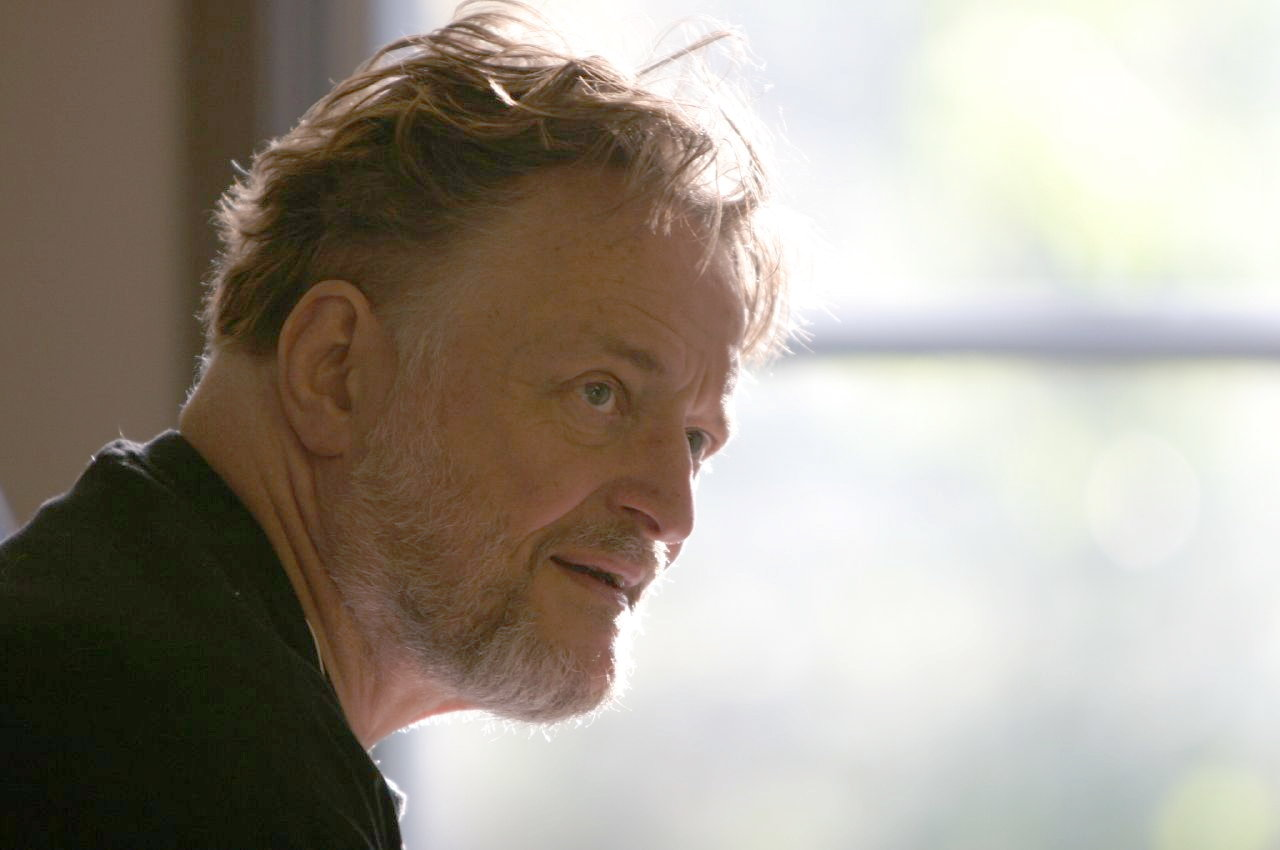
\includegraphics[width=8cm]{img/conway}\\

\footnotesize \textit{John Horton Conway}
\end{center}
\section*{\'Etape 1}

La suite de Conway est une succession de lignes obtenue très simplement :
\begin{itemize}
	\item 	On part de la ligne 0, qui vaut « 1 ».
	\item 	Chaque ligne est obtenue en \textit{décrivant} la ligne précédente.\\
            Par exemple, en décrivant la ligne 0, il y a un 1, ce qui donne « 1 1 » et c'est la ligne 1.\\
            La ligne 2 s'obtient de même : en décrivant « 1 1 » on obtient « 2 1 » et ainsi de suite.
\end{itemize}


\begin{questionnum}
    \'Ecrire les 7 premières lignes de la suite de Conway et vérifier que la ligne 6 est « 1 3 1 1 2 2 2 1 ».
\end{questionnum}

\begin{questionnum}
    \begin{itemize}
        \item 	Expliquer pourquoi il est impossible d'obtenir le nombre 0 dans une ligne.
        \item 	Expliquer pourquoi il est impossible d'obtenir le nombre 4 dans une ligne. 	
    \end{itemize}        
\end{questionnum}


\textit{On considère maintenant comme acquis le fait que sur chaque ligne il n'y a que des 1, des 2 et des 3.}\\
\newpage
La fonction suivante:
\begin{itemize}
	\item 	prend en entrée une liste d'entiers qui est une ligne de la suite de Conway ;
	\item 	renvoie la ligne suivante.
\end{itemize}

\begin{questionnum}
Complète sur ta copie le pseudo-code de cette fonction
\begin{verbatim}
    fonction conway(L : liste d'entiers)
        
        variables
        
            valeur, compteur, i , n : entiers
            resultat : ............
        
        début
            n ← longueur(............)
            resultat ← liste vide
            valeur ← L[0]    
            compteur ← 0     
            pour i allant de ............ à ............
                si L[i] = ............
                    compteur ← 
                sinon
                    resultat.ajoute(compteur)
                    resultat.ajoute(............)
                    valeur ← L[i]
                    compteur ← 1
                finsi
            finpour
            resultat.ajoute(............)
            resultat.ajoute(valeur)
            renvoyer resultat
        fin
    \end{verbatim}
\end{questionnum}


On aimerait savoir si le motif « 3 3 » apparaît dans la suite (en vérité, c'est le cas).

\begin{questionnum}
\'Ecrire le pseudo-code de la fonction \pythoninline{contient33} qui
\begin{itemize}
	\item 	en entrée prend une liste d'entiers ;
	\item 	renvoie un booléen indiquant si cette liste contient deux 3 consécutifs.
\end{itemize}

\end{questionnum}


\begin{questionnum}
    \'Ecrire le pseudocode de l'algorithme qui détermine la première ligne de la suite de Conway qui contient deux 3 consécutifs.
\end{questionnum}

\section*{\'Etape 2}

Le fichier \pythoninline{conway.py} contient le début de la fonction \pythoninline{conway} à compléter.

\begin{questionnum}
    Complète la fonction.
\end{questionnum}




\begin{questionnum}
    \'Ecris la fonction \pythoninline{contient33}.
\end{questionnum}


\begin{questionnum}
    \'Ecris le programme qui détermine la première ligne où deux 3 consécutifs apparaissent.
\end{questionnum}




\end{document}